% Create a sciposter with a size of 420 x 594 (DIN A 2)
% \documentclass[a2, plainboxedsections, draft]{sciposter}
% \documentclass[a2, plainboxedsections]{sciposter}
\documentclass[a2, plainboxedsections, final]{sciposter}

% Import Packages
\usepackage{multicol}   % Use multiple columns
\columnsep=2cm        % Space between columns
\columnseprule=1pt      % Width of the line inbetween the columns

\usepackage{tikz}       % Nice Graphs
\usepackage{listings}   % Code
\usepackage{array}      % Nice tables
\usepackage{times}      % Times New Roman
\usepackage{graphicx}   % Insert Images
\usepackage[english,ngerman]{babel}     % German symbols (ä, ö, ü, ß)
\usepackage[utf8]{inputenc}             % UTF-8

% title
\title{Galaxy Generation}               % Title of the Project
\author{Emile Hansmaennel}              % Name of the author
\institute{Theodor Fliedner Gymnasium}  % Institute
\email{emile.hansmaennel@gmail.com}     % Email
\leftlogo[1.25]{figs/galaxy}            % Logo left of the title
\rightlogo[1]{figs/logos_box}           % Logo right of the title

% Custom section header style
\usepackage{sectsty}
\sectionfont{\color{black}\itshape\selectfont\sectionrule{0pt}{0pt}{-4pt}{1pt}}

% footnote
\conference{\\ \textbf{Jugend Forscht 2018}, Emile Hansmaennel, Theodor-Fliedner-Gymnasium}

% Rest
\setmargins[2cm] % Page Margin

\begin{document}
  \maketitle

  \begin{multicols}{2}

  \begin{abstract}

  Das Ziel meines Projektes war es, Galaxien drei-dimensional zu
  visualisieren.
  Dazu verwendete ich das sogenannte ''Navarro-Frenk-White''' Profil als
  Dichtefunktion in Kombination mit der Random-Sampling Methode zum Generieren
  von Koordinaten.
  \par
  Die Generierung der Koordinaten hat jedoch ein Problem: Es ist extrem
  rechenaufwendig. Um dieses Problem zu lösen, habe ich mehrere Methoden zur
  Optimierung angewendet, darunter die Nutzung von Lookup-Tabellen und die
  Verwendung von mehreren Computer-Rechenkernen.
  \par
  Im Verlauf des Projektes habe ich viel Neues dazugelernt, darunter die
  Handhabung mit großen Datenmengen und die Organisation eines größeren Projektes,
  jedoch auch mit vielen tiefer gehenden Funktionen und Bibliotheken
  in der Programmiersprache Python umzugehen.

\end{abstract}


\vspace{0.5cm}
\setlength{\fboxsep}{10pt}
\fbox{
  \parbox{0.95\linewidth}{
  An das Praktikum im Astronomischen Recheninstitut in Heidelberg gelangte
  ich, indem ich mein Jugend Forscht Projekt aus dem letztem Jahr (Satellite
  Computation), auf der Social-Media Plattform Reddit hochgeladen habe, wonach
  mich der Doktorand Tim Tugendhat anschrieb, ob ich Interesse an einem
  Praktikum hätte, das ich im Sommer 2017 absolviert habe.
  }
}

  \section*{Hauptziele}

\begin{enumerate}
\item Generieren von elliptischen Galaxien mithilfe des Narvarro-Frenk-White-Profils in Verbindung mit der Random-Sampling Methode

\item Verbesserung des Generierungsprozesses mithilfe verschiedener Methoden
\begin{itemize}
  \item Lookup-Tabellen
  \item Unterteilung der Galaxie in verschiedene Zellen
  \item Effizientere Speichernutzung
\end{itemize}

\item Generierung von Dunkle-Materie-Halos und Spiralgalaxien

\item Nutzung von konkurrierenden neuronalen Netzen zum unbeaufsichtigten
Generieren von Galaxien und deren Anpassung an ''echte`` Galaxien.
\end{enumerate}

  \section*{Nutzen}

\begin{itemize}
  \item Visualisierung zur Verbesserung der Vorstellung von Galaxien

  \item Möglichkeit, sich eine Galaxie aus allen Perspektiven
  anzusehen

  \item Modell einer Galaxie, welches genutzt werden kann, um Vorhersagen
  für die echte Galaxie zu treffen
\end{itemize}

  \section*{Methoden}

\begin{itemize}
  \item Random Sampling des NFW-Profils
  \item Generierung von Lookup-Tabellen
  \item Code Vectorization
  \item Parallelization
  \item Kräfteberechnung mithilfe der universellen Gravitationsformel
\end{itemize}

  \section*{Random-Sampling des NFW Profils}

Beim Random-Sampling wird eine zufällige Koordinate generiert und dessen
Abstand zum Mittelpunkt der Galaxie \( r \) berechnet.
Diesen Wert \( r \) setzt man in das NFW-Profil ein, um eine Wahrscheinlichkeit
\( \phi = \rho(r) \) zu berechnen, mit der der Stern generiert wird.
Es wird ein zufälliger Wert \( s \) im Intervall \( [\rho_{min};~\rho_{max}] \)
generiert.
Gilt \( s < r \), dann werden die Koordinaten des Sterns beibehalten,
ansonsten werden neue Koordinaten generiert und der Prozess wird wiederholt.

\begin{center}\vspace{-1cm}
\begin{equation} \label{eq:NFW_profile}
  \rho_{NFW}(r) = \frac{ 1 }{ \sqrt{ 2 \pi } \cdot \sigma } \cdot
  \exp \left( \frac{ -\phi(r) }{ \sigma^{ 2 } } \right)
\end{equation}

\begin{equation}
  \phi(r) = \frac{ 4\pi \cdot G \cdot f_{0} \cdot R_{s}^3 }{ r } \cdot
  ln{ \left( 1 + \frac{ r }{ R_{s} } \right) }
\end{equation}
\end{center}%\vspace{0.5cm}
%
\begin{center}\vspace{-0.5cm}
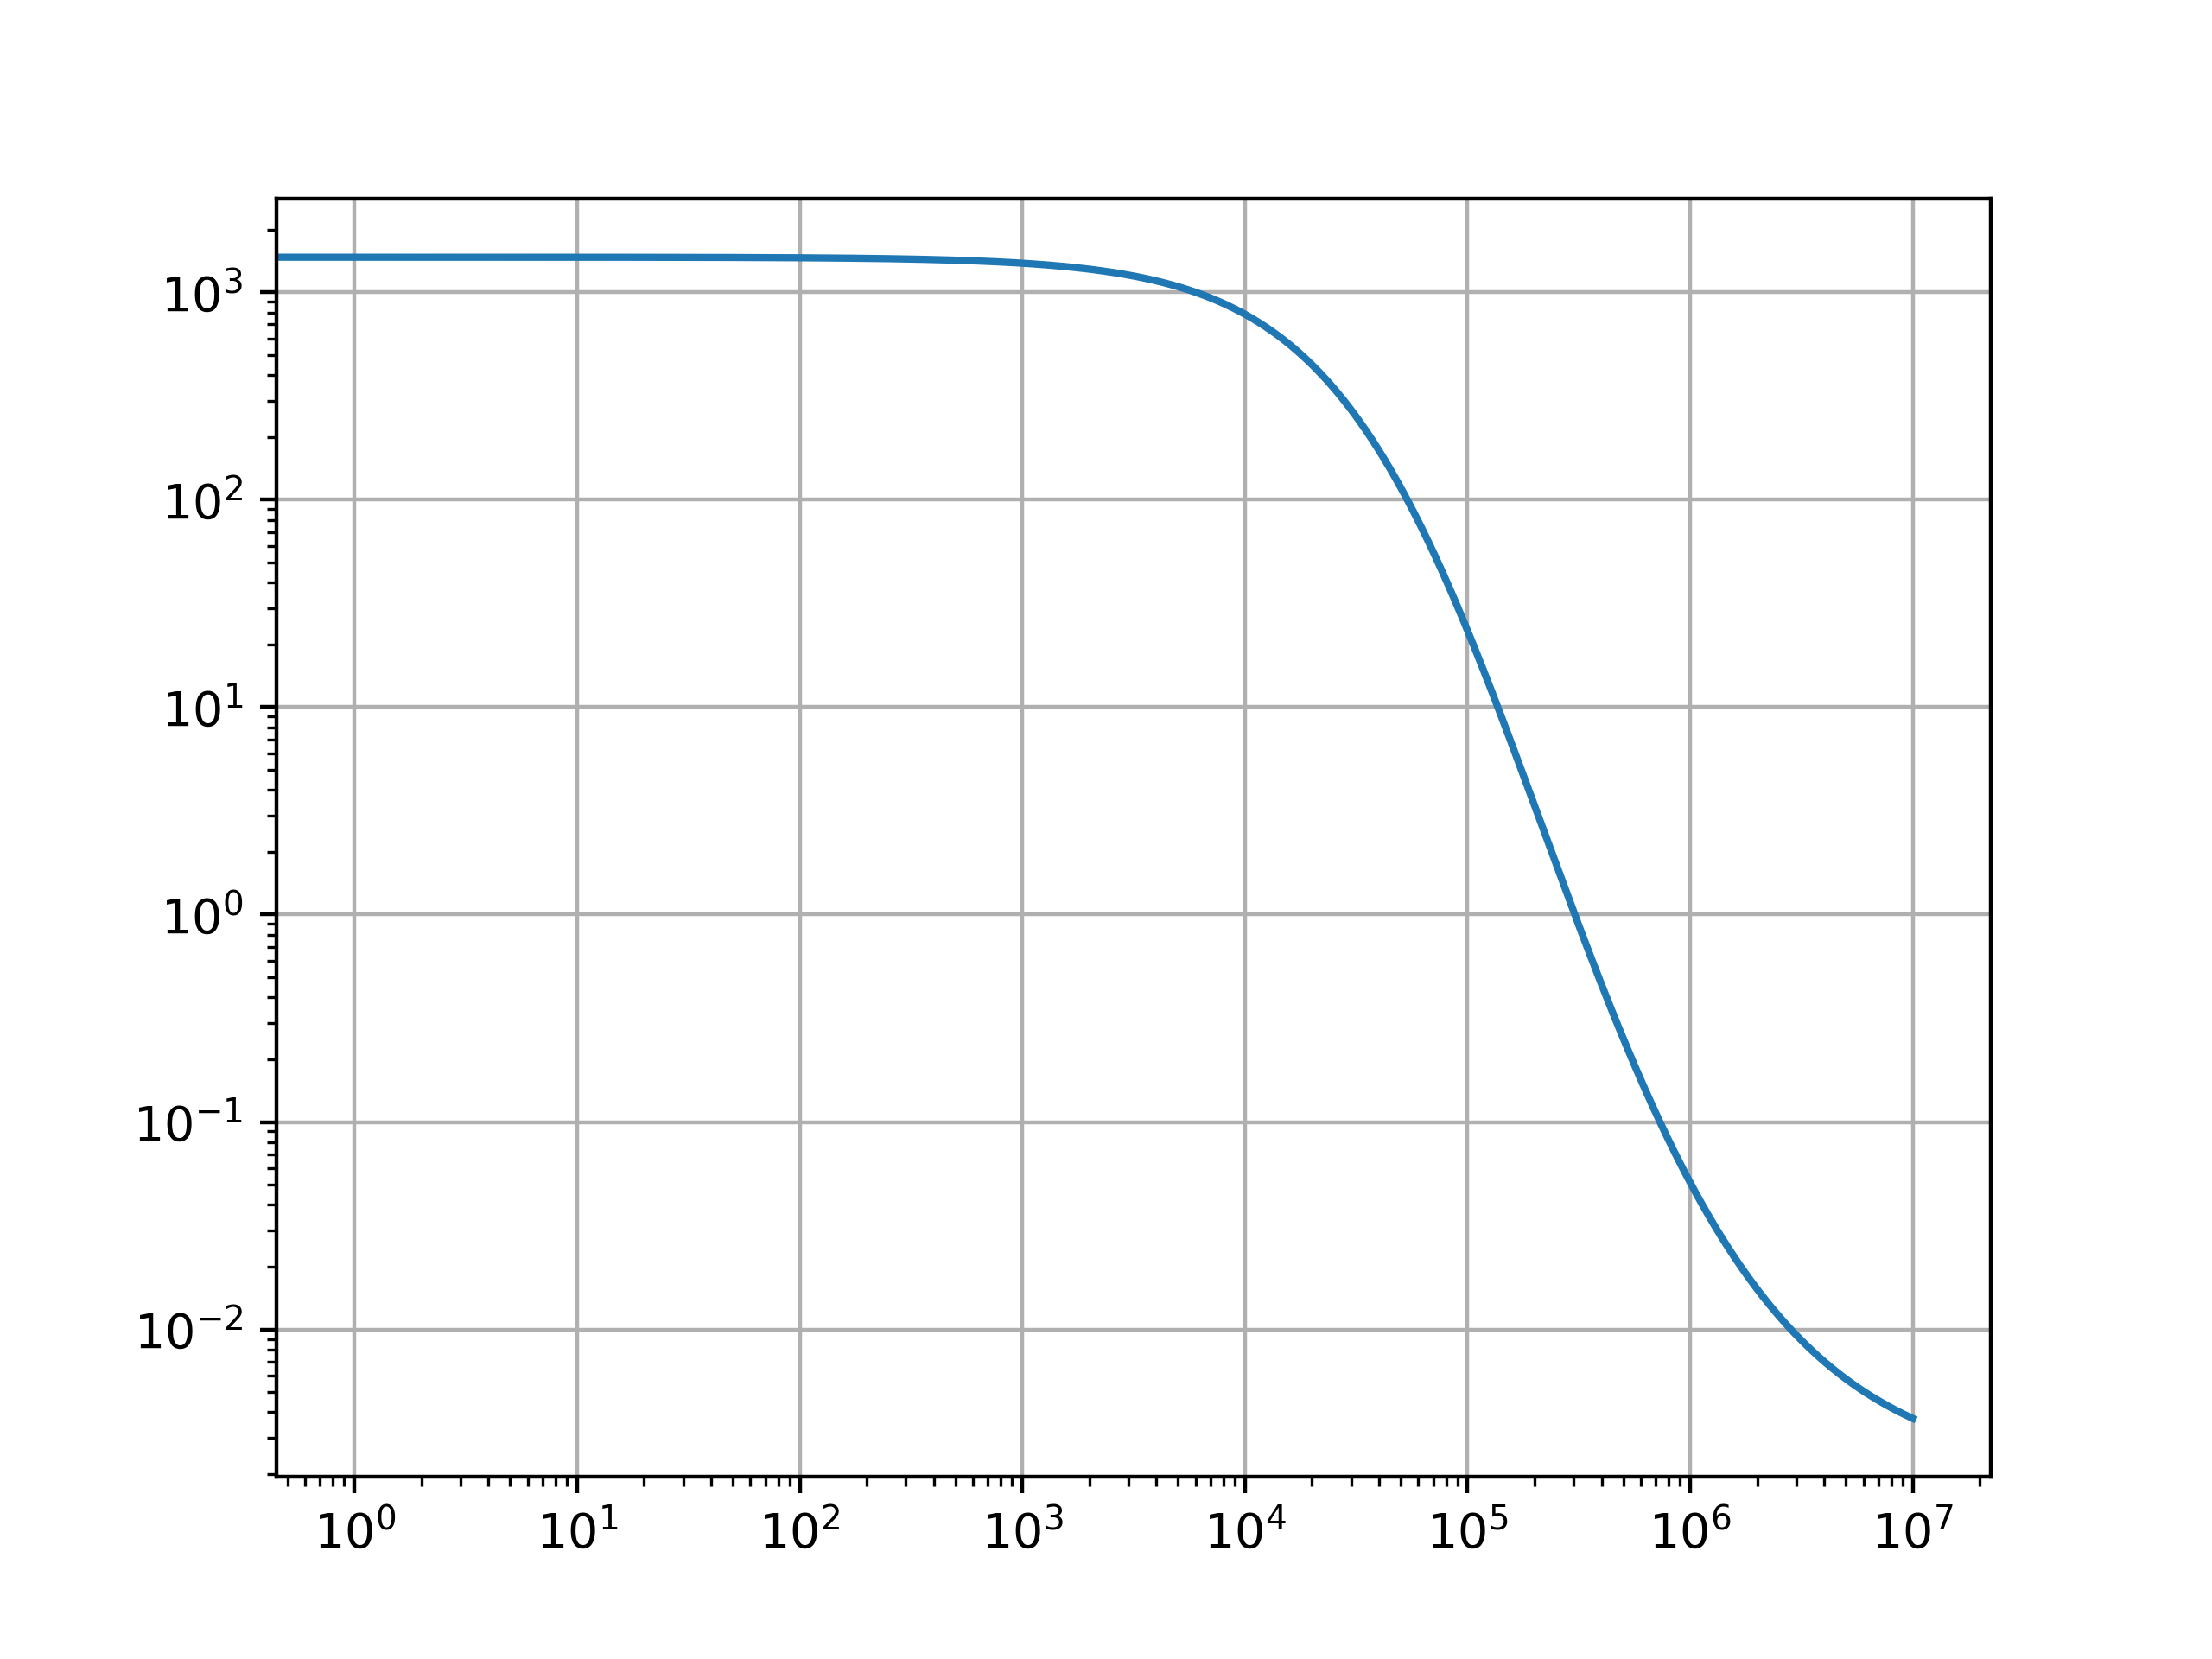
\includegraphics[width=0.8\linewidth]{figs/1e6_6}
\caption{Der entsprechende Funktionsgraph zum NFW-Profil}
\label{fig:lookup_NFW}
\end{center}\vspace{-1cm}

  \section*{Lookup Tabellen}

Um den Rechenaufwand der beim Berechnen eines Wertes aus dem NFW-Profil
entsteht zu mindern, wird die Funktion \( \rho(r)\) im Vorhinein
berechnet und zum Weiterverwenden gespeichert:

\lstset{
  frame=single,
  % numbers=left,
  title=2e8.csv \qquad (\( \sim \) 500 MB)
}

\begin{lstlisting}
0, 1477.1586582000994
1, 1477.0588424006478
2, 1476.9590343243835
3, 1476.8592346184294
4, 1476.7594429495975
...
19999995, 0.0028544345590963767
19999996, 0.0028544345175450904
19999997, 0.0028544344759938085
19999998, 0.002854434434442531
19999999, 0.002854434392891257
\end{lstlisting}

Möchte man zu einem Wert \( r \) aus der Funktion die Wahrscheinlichkeit
\( \rho(r) \) erhalten, muss man nur noch aus der Tabelle ablesen.
\par
Hier entsteht jedoch ein Problem: Alle Prozesse müssen aus dieser Tabelle die
Werte auslesen, weshalb sie für jeden Prozess einmal in den Arbeitsspeicher
geladen werden müssen. Dies lässt sich jedoch durch effizientes Parallelisieren
umgehen.

  \section*{Rechenaufwand (n-Körper Problem)}

\begin{equation}
  O(n) = n^2 \quad \Rightarrow \quad O(n) = n \cdot log(n)
\end{equation}

Um die Kräfte die zwischen allen Sternen in einer Galaxie wirken zu berechnen
werden \( n^2 \) Rechenschritte benötigt (\( n \) entspricht der Anzahl der)
Sterne.

\vspace{-0.25cm}
\begin{center}
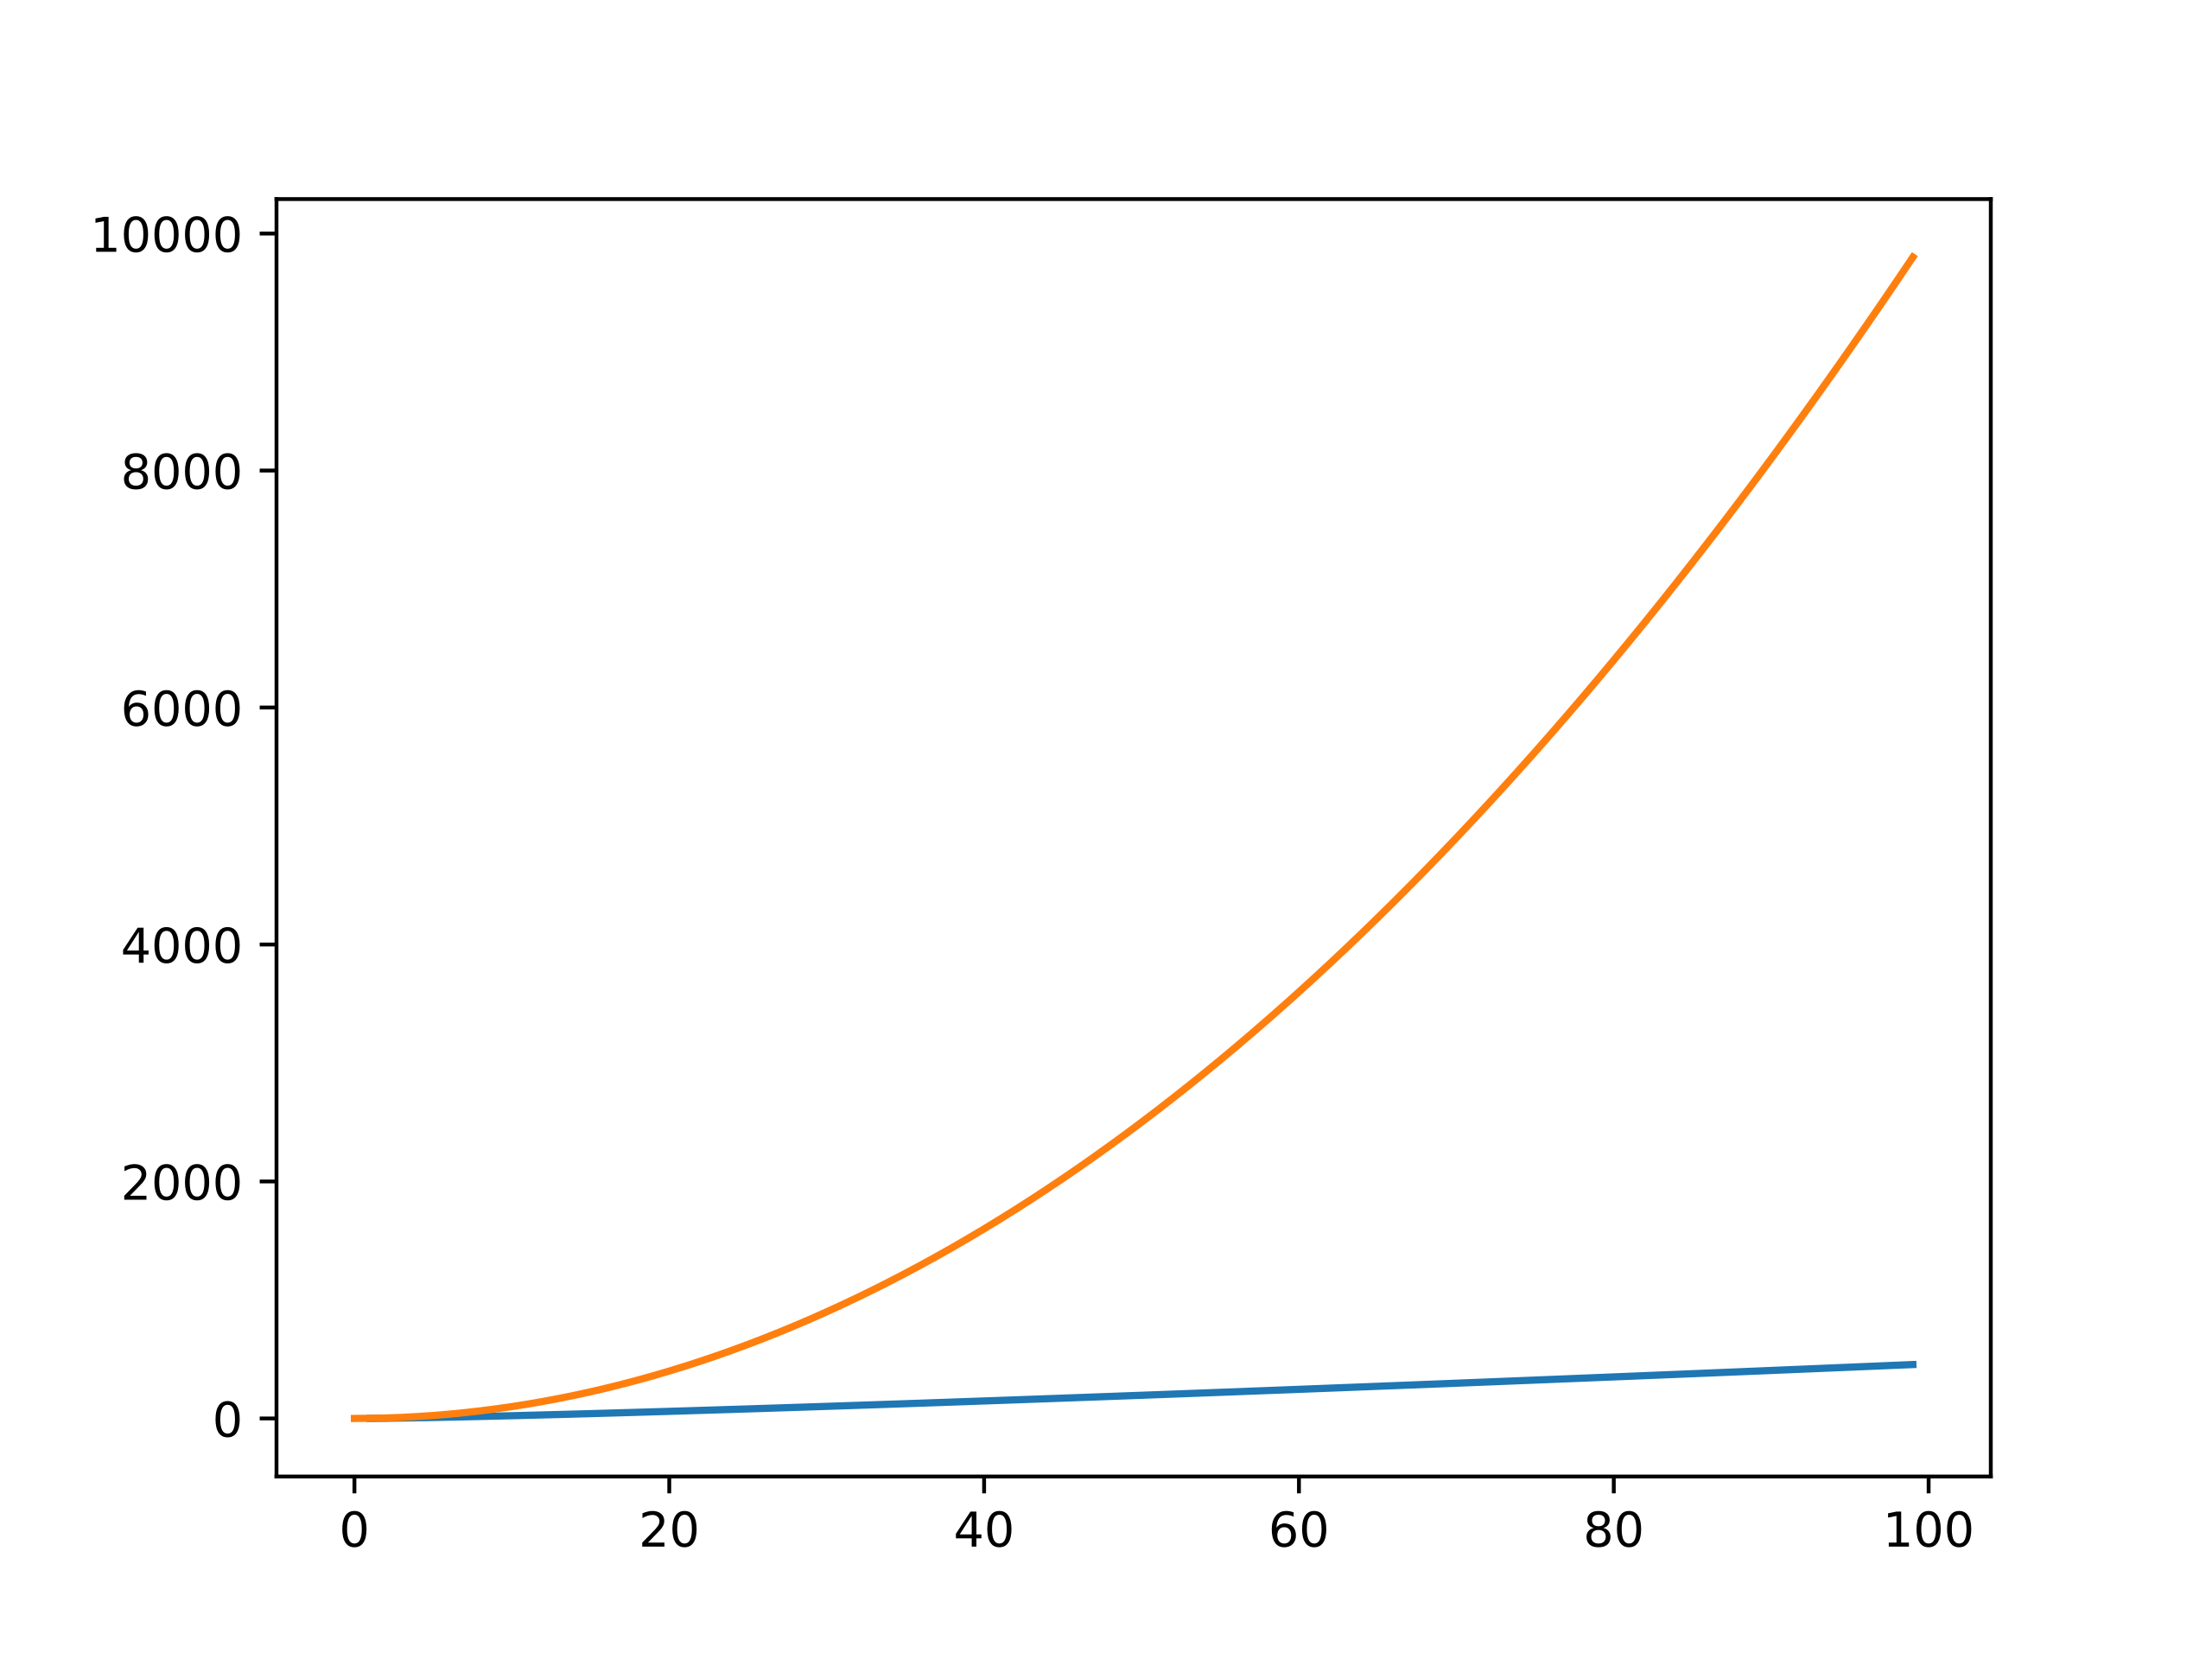
\includegraphics[width=0.8\linewidth]{figs/bigo_large}
\caption{Orange \( n^2 \), Blau \( n \log(n) \)}
\label{fig:bigo}
\end{center}\vspace{-1.25cm}

  \section*{Kräfte die auf einen Stern wirken}

Um die Gesamtkraft die auf einen Stern wirkt zu berechnen, habe ich
das Newton'sche Gravitationsgesetz in der folgenden Form verwendet:

\begin{equation}
  \vec{F_1} = G \cdot m_1 \cdot \sum_{i=2}^n m_i \cdot
  \frac{\vec{r_i} - \vec{r_1}}{| \vec{r_i} - \vec{r_1} |^3}
\end{equation}\vspace{-1cm}

  \section*{Unterteilung der Galaxie in Zellen}

Um den Rechenaufwand, der bei der Berechnung der wirkenden Kräfte entsteht,
zu minimieren, wird die Galaxie in verschiedene Zellen unterteilt:

\begin{center}\vspace{1cm}
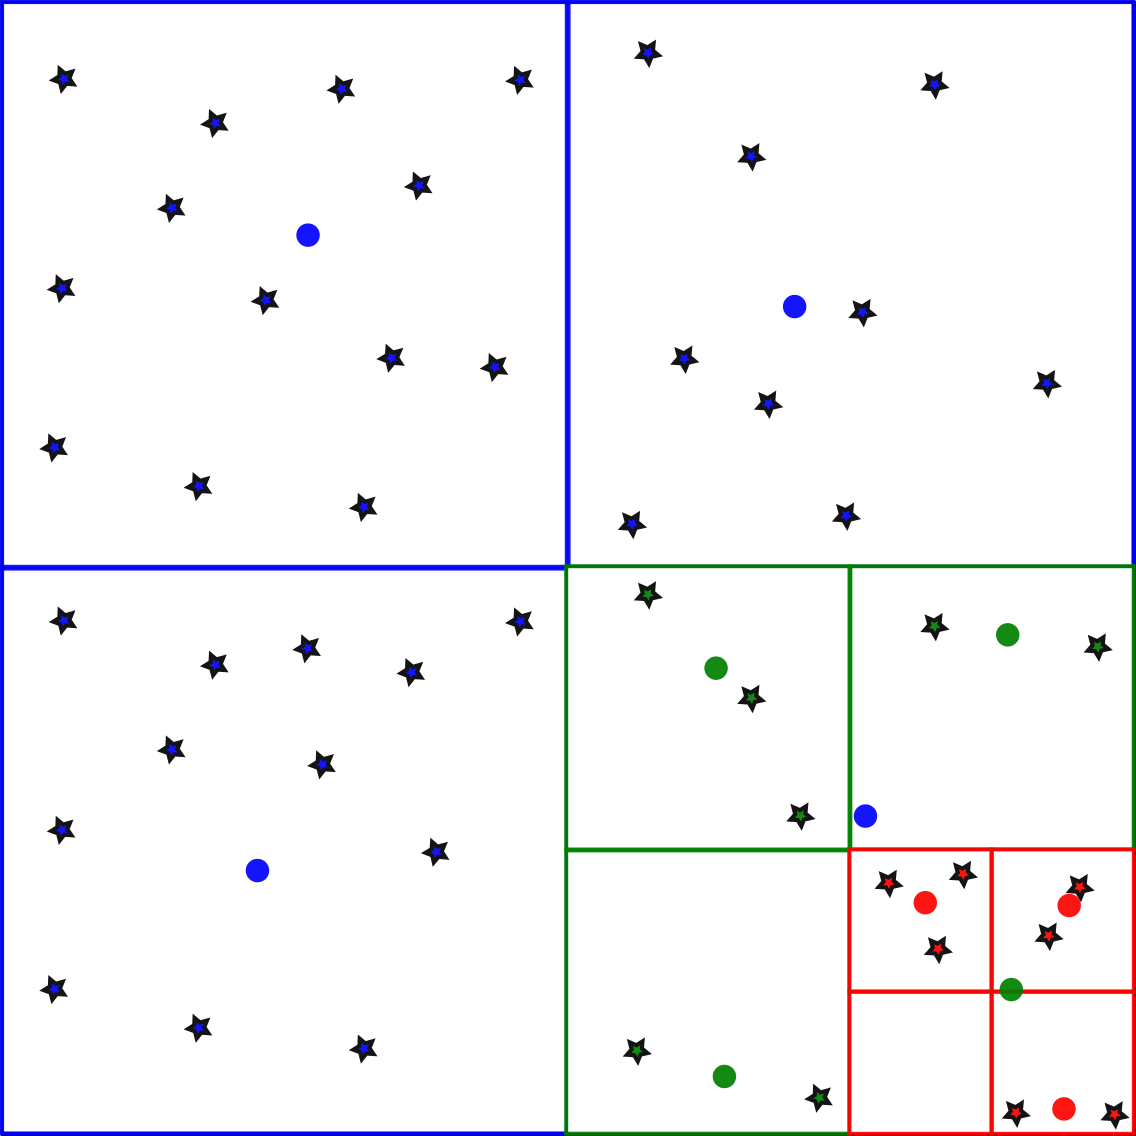
\includegraphics[width=0.8\linewidth]{figs/cells_2D}
\label{fig:galaxy_cells}
\end{center}

\begin{center}
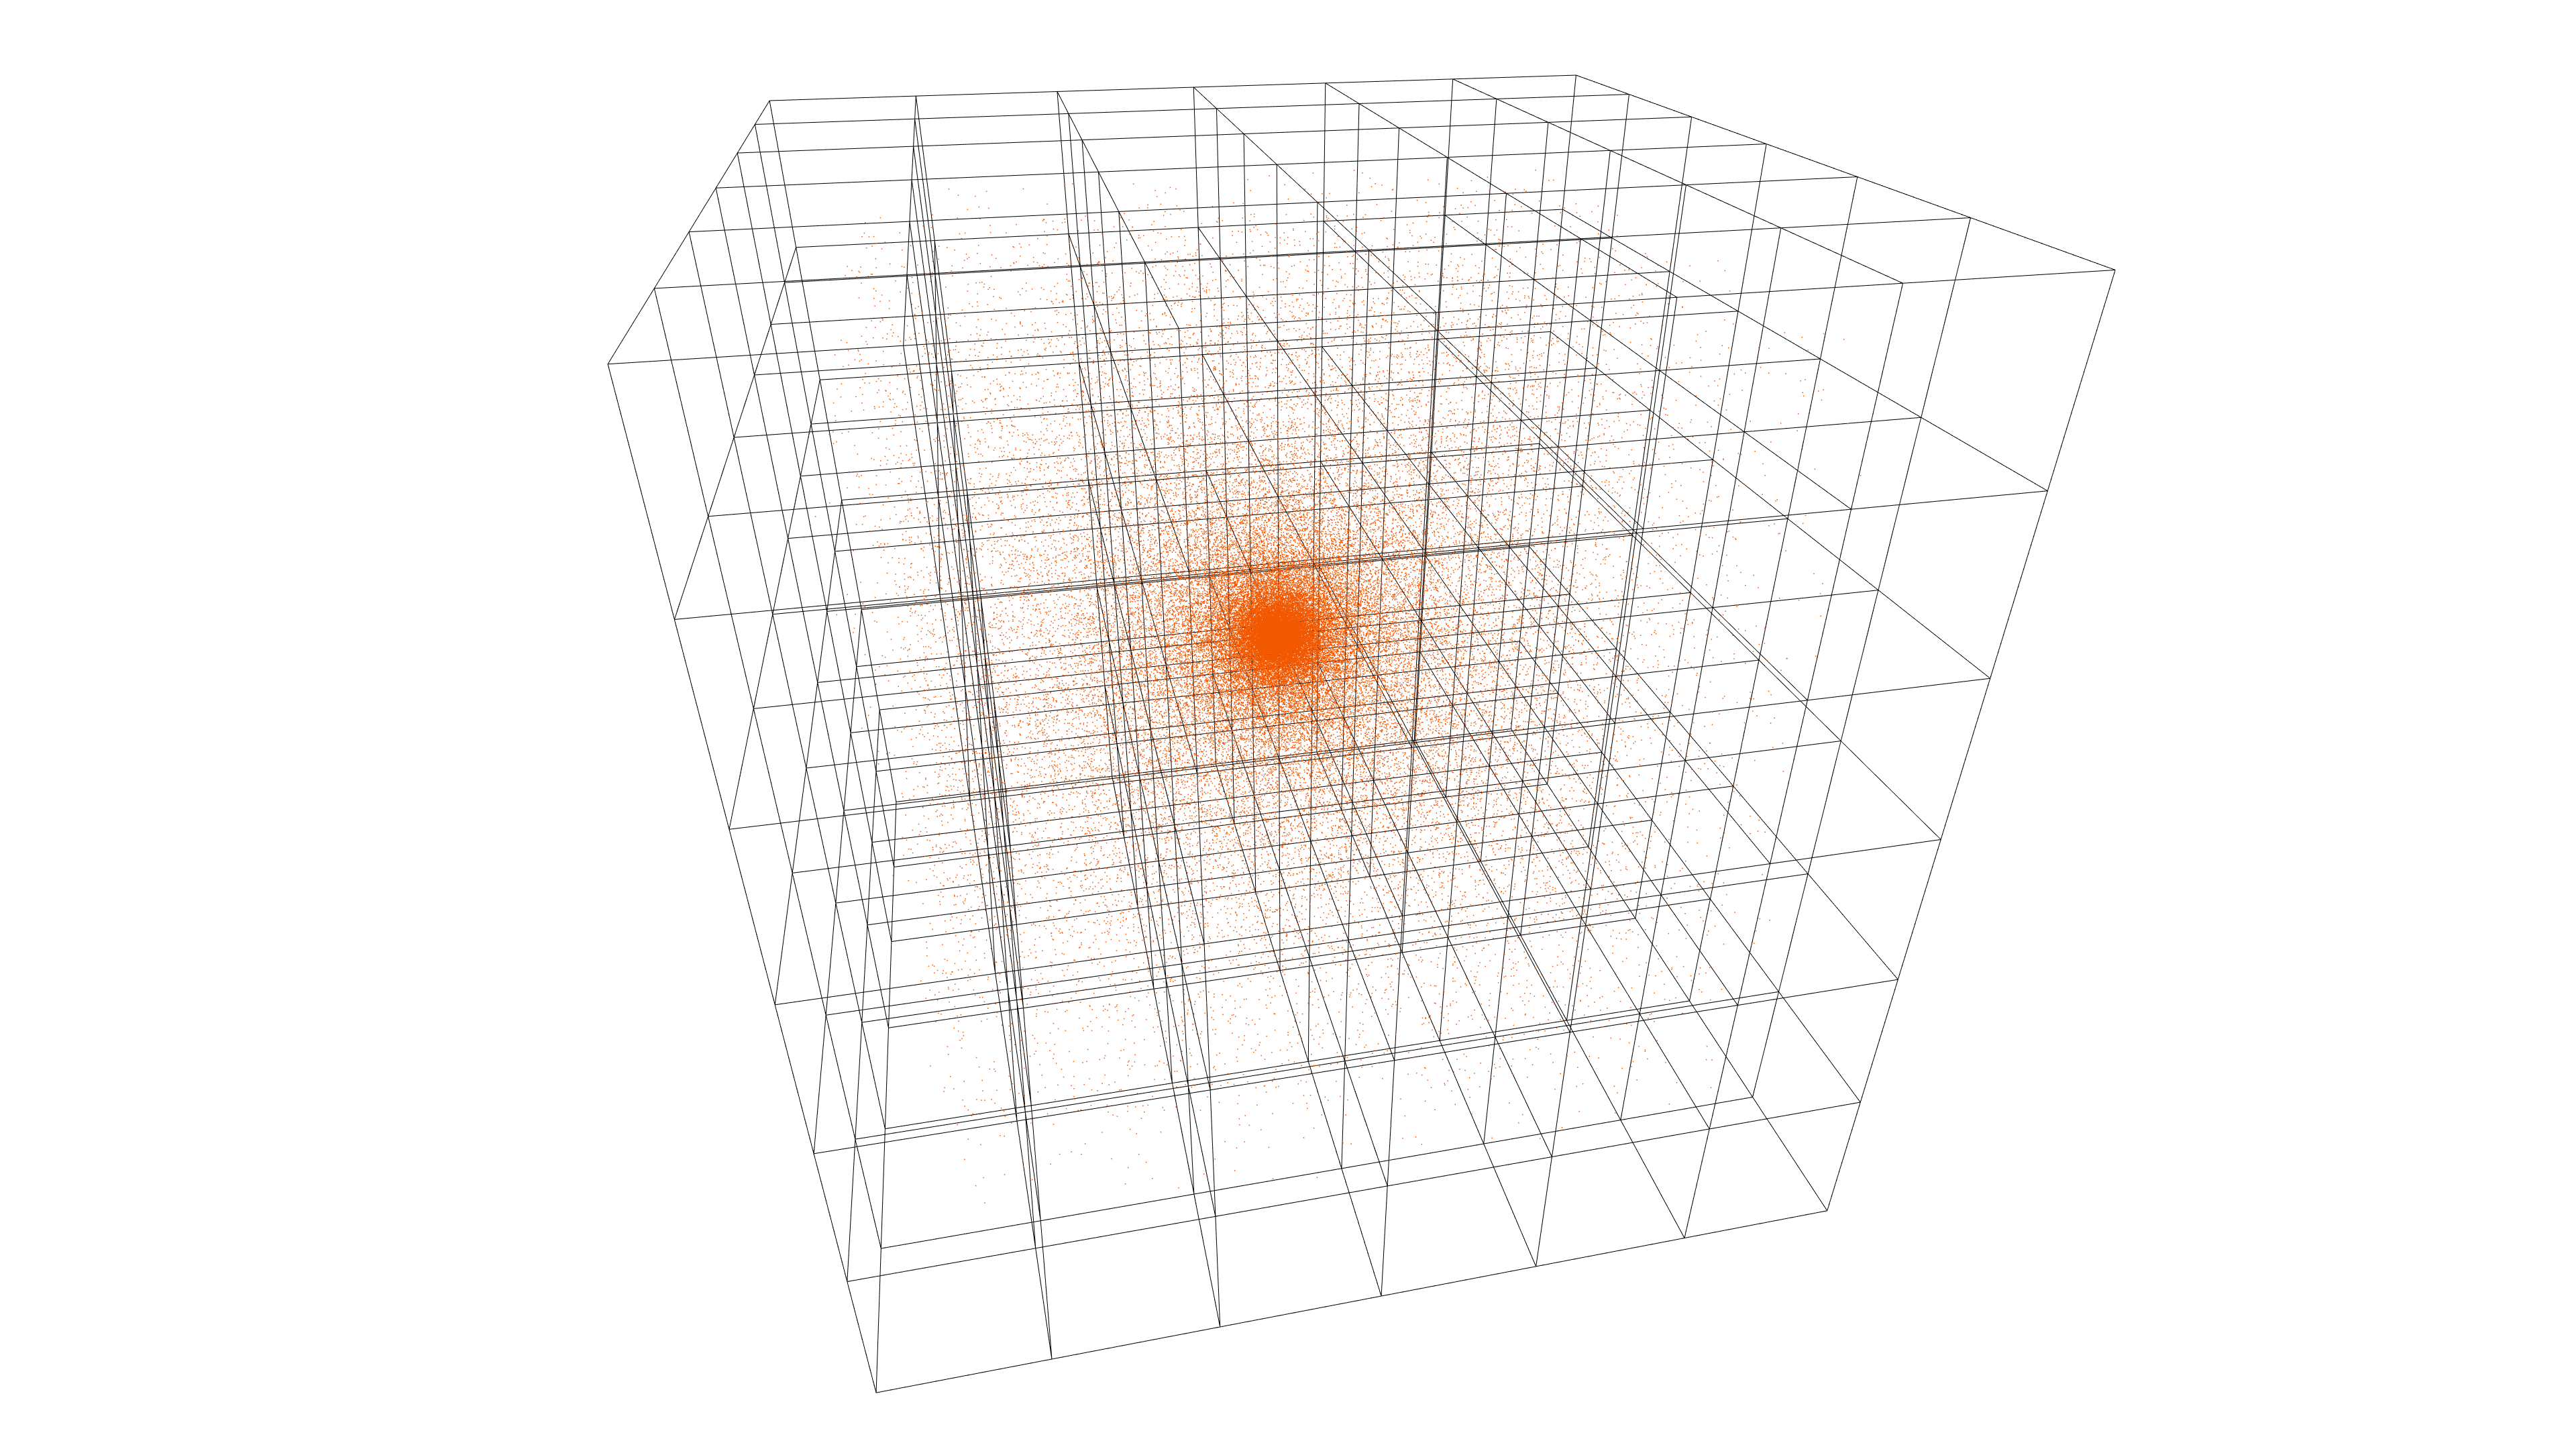
\includegraphics[width=1\linewidth]{figs/cells}
\label{fig:galaxy_cells_3d}
\end{center}\vspace{-3cm}

  \section*{Genutzte Rechner}

{\setlength{\extrarowheight}{10pt}%
\begin{tabular}{l | l | l | l}
  Bezeichnung         & Kerne  & Threads & Taktrate \\[0.25ex] \hline
  Acer Laptop         & 2      & 4  & 3.1 GHz \\
  Heidelberg Cluster  & 44     & 88 & \( \sim \) 2.5 GHz \\
  Flammkuchenblech    & 6      & 24 & 2.5 GHz \\

\end{tabular}
}

  \section*{Generative Adversarial Neural Networks}

\begin{center}\vspace{0.5cm}
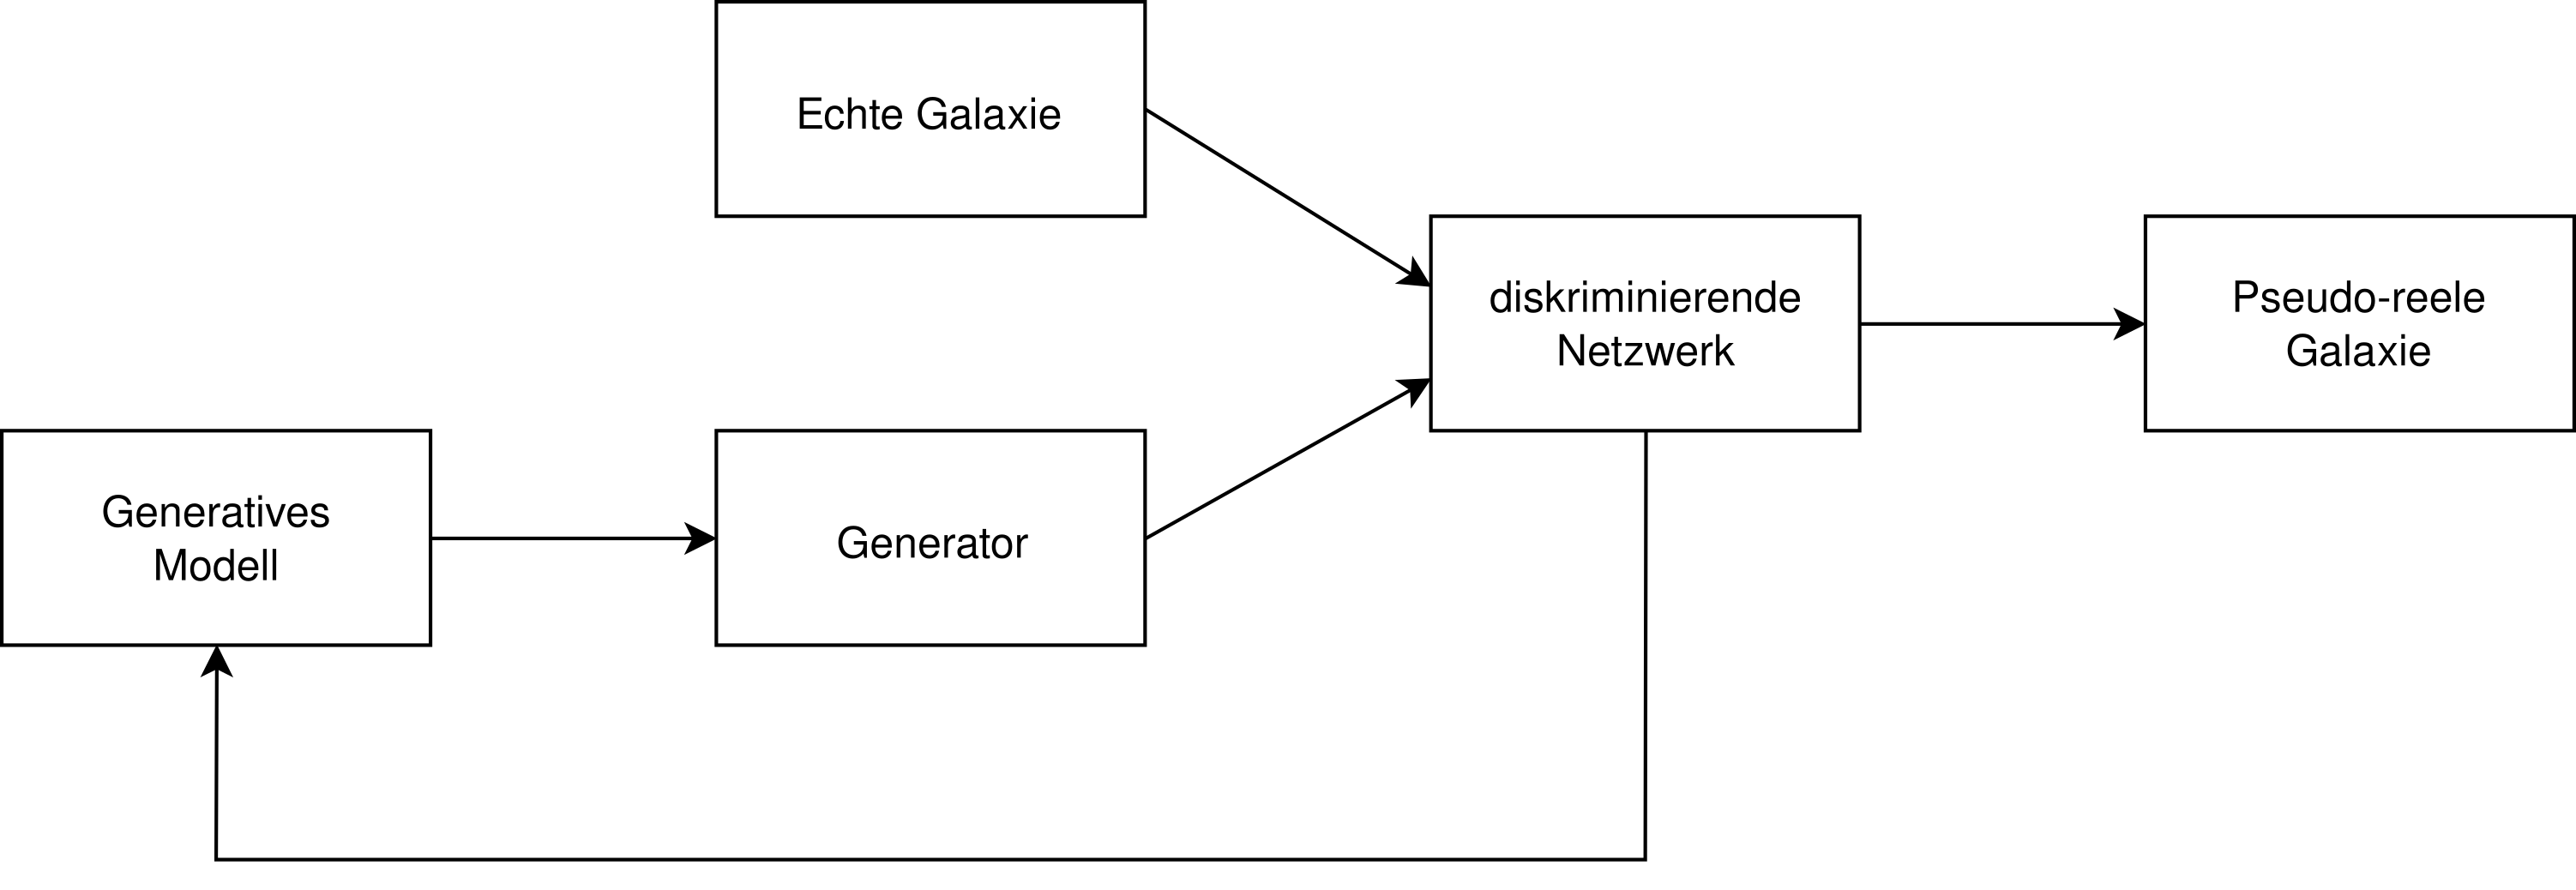
\includegraphics[width=1\linewidth]{figs/galaxy_gan.png}
\caption{Aufbau eines GAN Netzwerkes zum Generieren von Galaxien}
\label{fig:galaxy_gan}
\end{center}\vspace{-1cm}

  \section*{Ergebnisse}

\begin{center}\vspace{0.5cm}
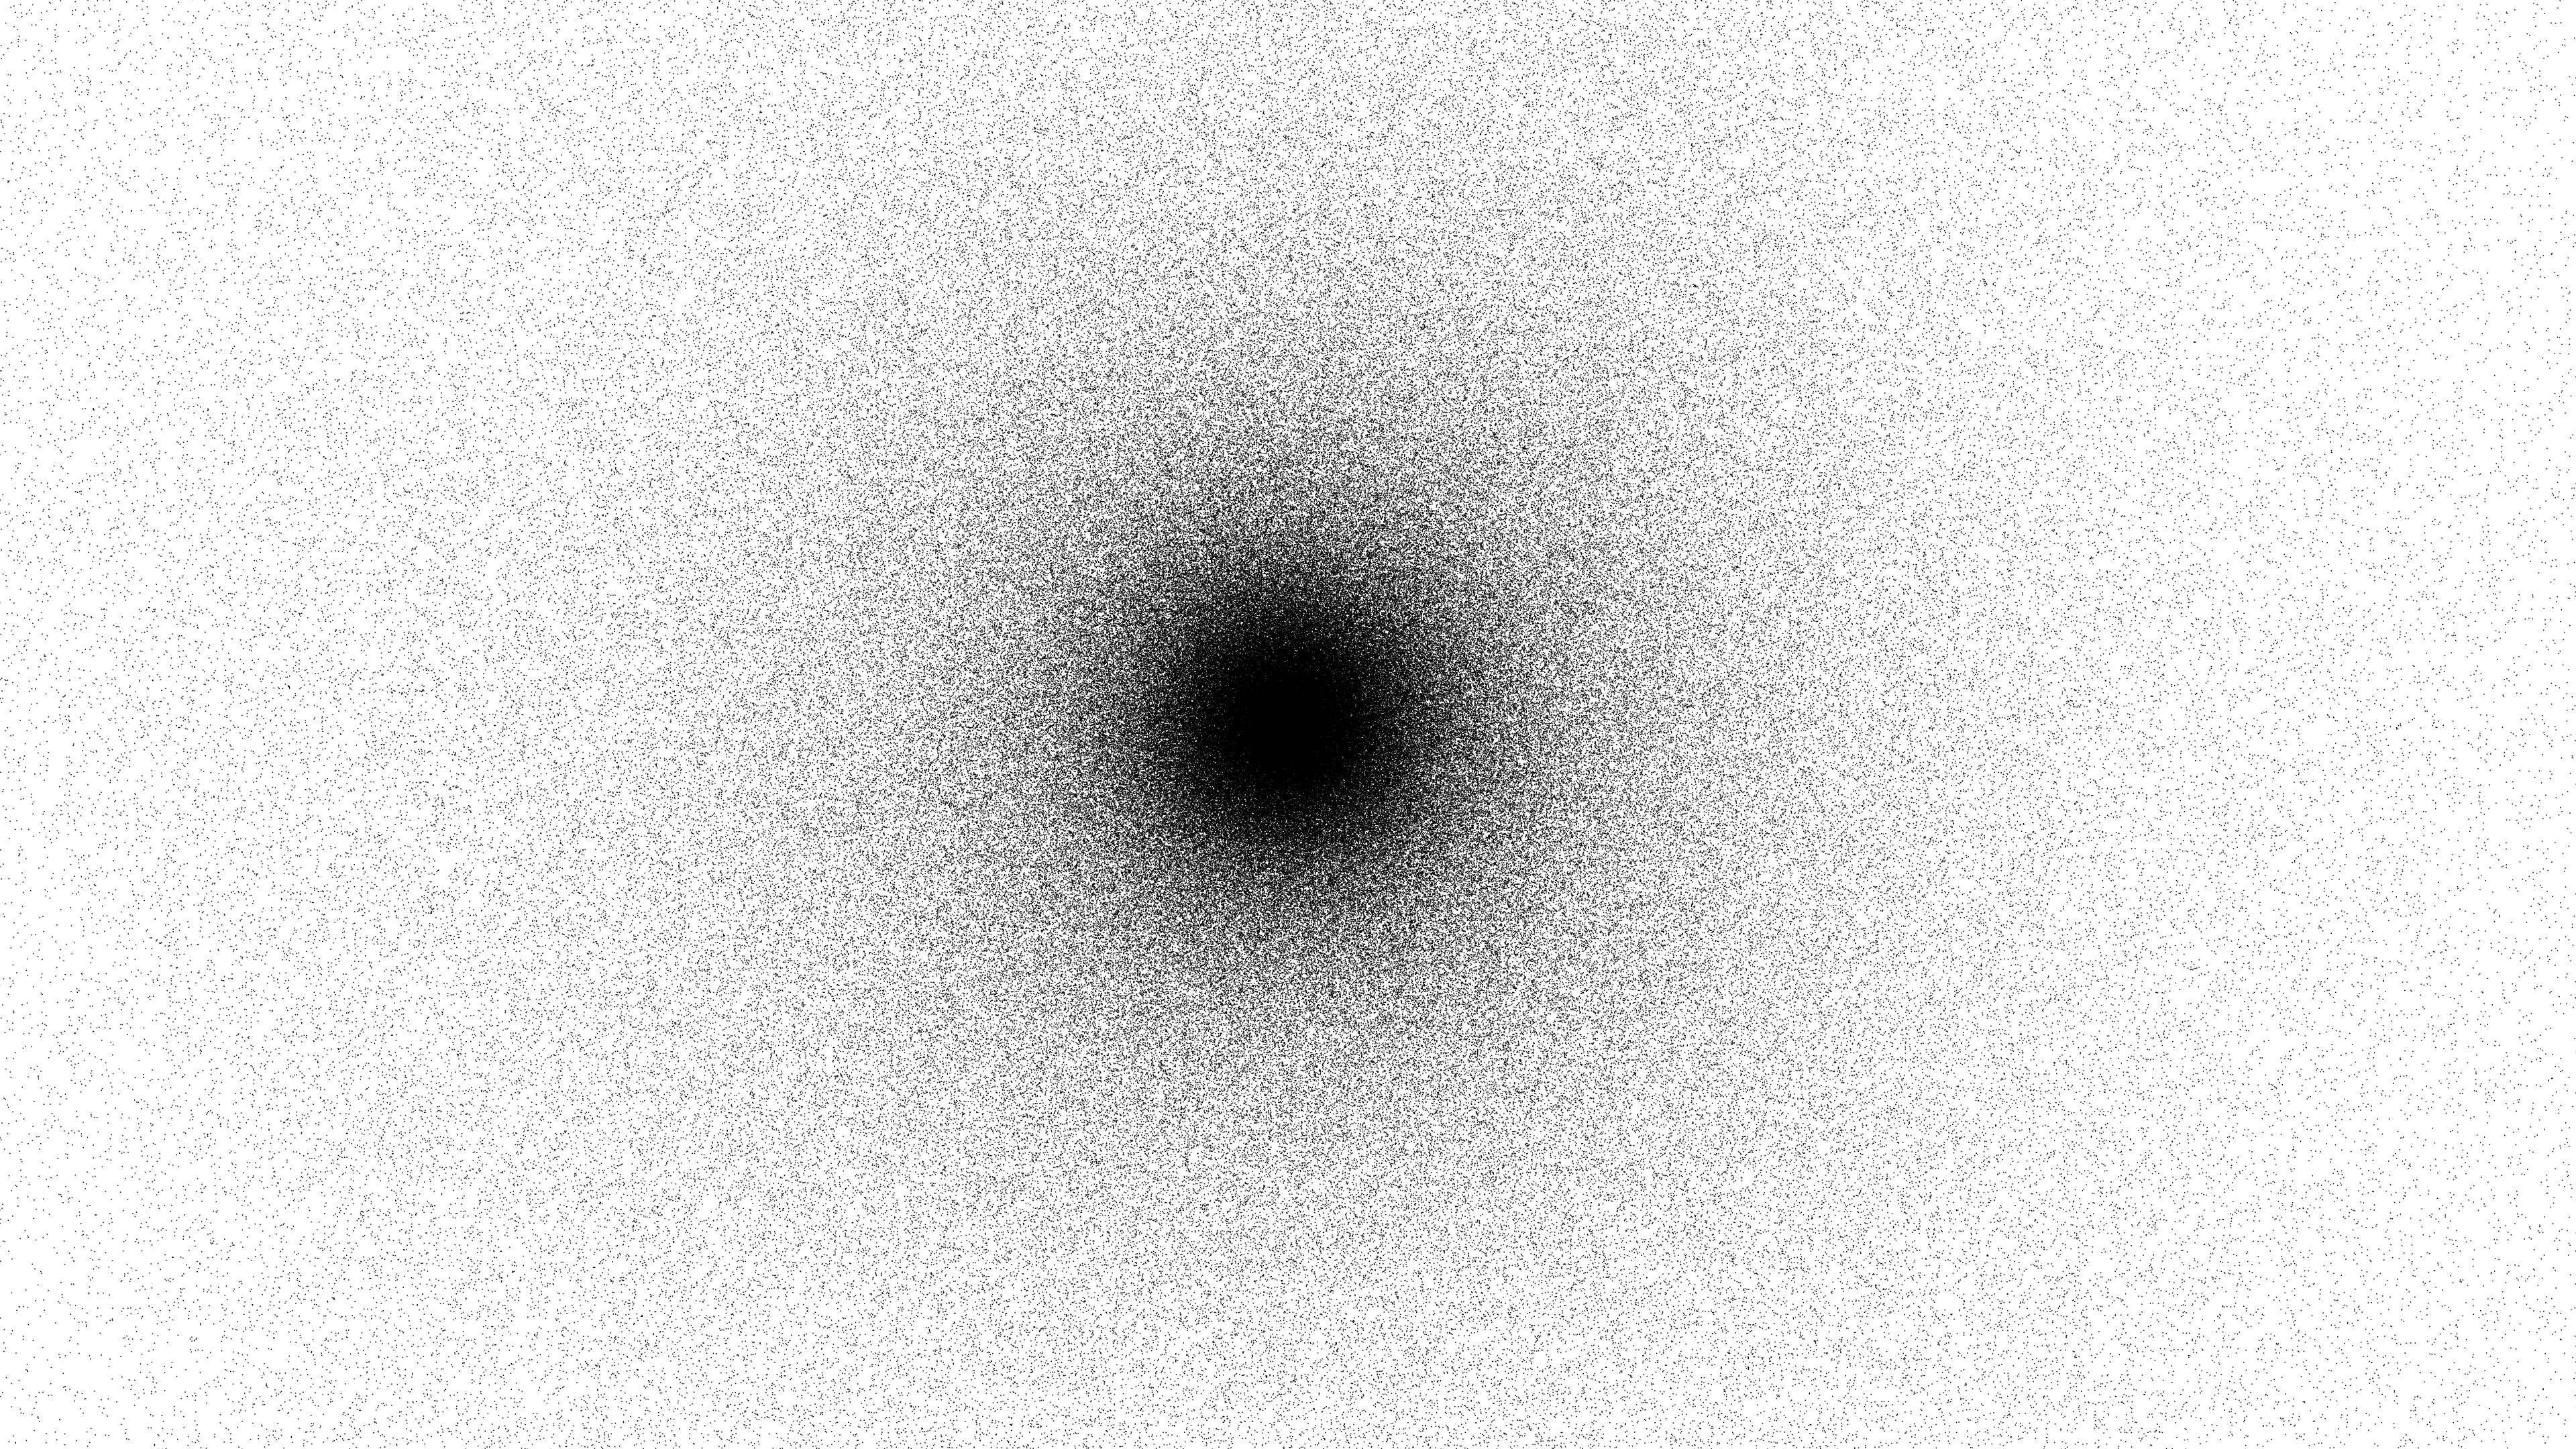
\includegraphics[width=0.8\linewidth]{figs/galaxy_flammkuchenblech}
\caption{ Diese generierte Galaxie bestehend aus \( 680.000 \) Sternen}
\label{fig:galaxy_flammkuchenblech}
\end{center}\vspace{-1cm}

  \section*{Zukunft}
\begin{itemize}
  \item OpenMP
  \item OpenACC statt CUDA oder OpenCL
  \item Code Vectorization
  \item Shared Memory
  \begin{itemize}
    \item[\( \rightarrow \)] Distributed Memory
  \end{itemize}
  \item Hilbert Spiral
  \item Nutzung des L1, L2 und L3 caches
\end{itemize}

  \section*{Danksagungen}

Hier möchte ich mich bei \( \dots \)
\begin{itemize}
  \item[\( \dots \)] Tim Tugendhat
  \item[\( \dots \)] Konstantin Bosbach
  \item[\( \dots \)] Jörg Thar
  \item[\( \dots \)] Martin Dessauer
\end{itemize}
bedanken, denn ohne sie wäre die Durchführung des Projektes nicht möglich
gewesen.

% Tim Tugendhat und Konstantin Bosbach bedanken ohne die
% das Praktikum in Heidelberg nicht möglich gewesen wäre, welches mir den einstieg
% in das Thema erst ermöglicht hat.


  \end{multicols}
\end{document}
